\subsection{Improving the performance of dynamic languages when executing data-driven tasks}
Dynamic, interpreted languages are commonly celebrated for their increased succinctness over static, compiled languages. Often, they greatly reduce the amount of code that is necessary to perform common tasks. However, they continue to be overshadowed by the throughput resultant from heavily optimised compilation of static languages, particularly for performance-intensive procedures. A typical performance divergence is shown in Figure~\ref{fig:ruby_vs_c}.

\begin{figure}[h]
  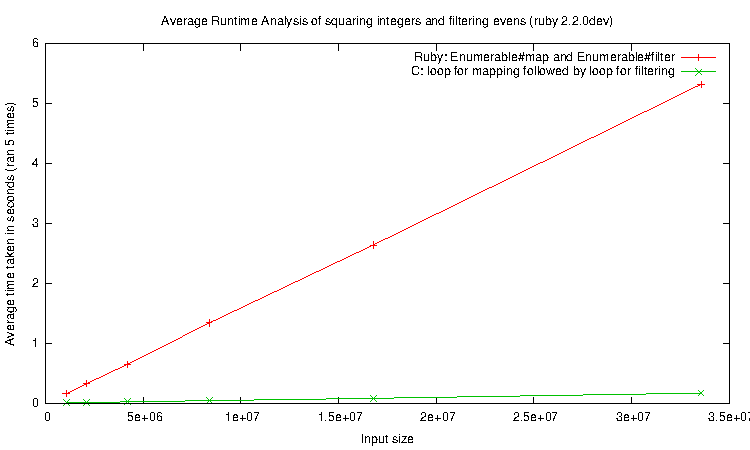
\includegraphics[width=\textwidth]{./figures/ruby_vs_c.pdf}
  \caption{Graph demonstrating the significant difference in performance when operating on large datasets in C and Ruby.}
  \label{fig:ruby_vs_c}
\end{figure}

RubiCL aims to investigate and mitigate any decreased performance experienced when using the Ruby language for data processing. By producing a more efficient implementation of computational tasks, users will be able to tackle larger scale problems without needing to learn new toolchains.

\paragraph*{Indicators of success}
Progress towards this goal can be evaluated by comparing the performance of data-driven computation tasks in Ruby, with and without the library's contributions, to that of functionality provided by native extensions written in static languages. Further success can be measured by investigating whether increased magnitude computation now terminates within reasonable time, due to the project's contributions.

\subsection{Facilitating a larger scale of experimentation in a REPL environment by non-expert users}

An interactive environment, such as a \ac{REPL}, is commonly useful for rapid prototyping. It allows online processing of data without the need to produce all of the required code upfront, as shown in Listing~\ref{lst:repl}. \acp{REPL} are absent from many languages. In supported languages, they allow the user to continuously query data and return intermediate results. Often, a quick turnaround between idea and response leads to more questions. This can enable an investigational attitude to computer programming.

\begin{lstlisting}[
  language=Ruby,
  label=lst:repl,
  caption=A basic example of using a REPL environment for data analysis.
]
dataset_1.mean
# =!> NoMethodError: undefined method `mean' for Array

module Enumerable
  define_method(:mean) { map(&:to_f).inject(&:+) / size }
end
#=> :mean

dataset_1.mean
#=> 23.6

dataset_2.mean
#=> 23.2
\end{lstlisting}

By widening the scope of problems that can be evaluated within a \ac{REPL}, RubiCL shall enable a larger scale of investigation. Analysis of particularly large datasets is currently unavailable to novice users, due to the amount of computation required.

\paragraph*{Indicators of success}
The completed library should be presented to novice analysts, users with mathematical insight but insignificant programming prowess. If they are able to easily answer queries about large datasets, the system's design will be judged as successful. As with the previous goal's evaluation, response time within a \ac{REPL} environment will be examined.

\subsection{Exploring the extensibility of the Ruby programming language}
Ruby has served as a suitable foundation for many \acp{DSL}, including build tools\cite{rake} and web frameworks\cite{sinatra}.

The language has open classes, whereby the structure of object classes can always be altered at runtime, even after definition ends. It also permits a variety of meta-programming techniques, allowing complicated code to appear misleadingly simple at the surface.

\begin{lstlisting}[
  language=Ruby,
  label=lst:sinatra,
  caption=The Sinatra DSL for simple web programming hides complexity when writing basic web services.
]
require 'sinatra'

get '/hi' do
  "Hello World!"
end
\end{lstlisting}

Objects in Ruby are often regarded as \emph{duck-typed}. This means that the system should care only about how an object behaves \textemdash{} ``If it looks like a duck, swims like a duck, and quacks like a duck, then it probably is a duck.''\cite{ducktest}

Since function invocation uses a \emph{method-sending} approach, the underlying implementation can be altered significantly as long as an expected dialog is presented to the runtime.

This project demonstrates integrating drastically different processing techniques into the language's runtime. It achieves this without greatly affecting the code that a user must write in order to use them.

\paragraph*{Indicators of success}
The integration will be successful if the interface for processing data remains consistent. Parallelism should be implicit and not requiring direction from the programmer. Again, user testing will evaluate this.

\subsection{Effective code generation and reuse on the OpenCL platform}
\ac{OpenCL} can provide high throughput computation, often utilised by bespoke systems such as cryptographic hashers and video encoders. However, there is a significant amount of configuration and set-up code associated with each parallel tasks performed. Code reuse is difficult to achieve on the \ac{OpenCL} platform due to the specificity of kernel execution.

Without techniques for reuse, advances made by one parallel project may not be applicable to others. In this case, programmers writing parallel systems must implement all subtasks from the bottom up when constructing the full solution. As it is hard to incorporate the partial solutions of others, barriers to entry are further increased.

This project undertaken will attempt to recycle the partial solutions of primitives as much as possible. This allows investigation into how much reuse is possible, given an ideal system with a single author.

With greater code reuse, optimisations of a given subtask will improve all primitives utilising the component. This directs experimentation when searching for performance improvements.

\paragraph*{Indicators of success}
Unfortunately, code reuse is often best measured subjectively. Yet, the developer's opinion when reflecting on the development experience may provide useful insight. If code reuse techniques facilitate the development of this particular \ac{OpenCL} project, it is likely that they may be beneficial to developers elsewhere.

\subsection{Applicability to a variety of platforms, avoiding over-tailoring for a specific machine}
The project should be packaged in a manner that facilitates installation onto a new, supported, system. In addition, it should achieve performance enhancement without having to be adjusted significantly by the user.

As a result, no assumptions about the specific hardware present can be made, apart from full \ac{OpenCL} support. This will allow the project to support a range of current and future compute-devices.

\paragraph*{Indicators of success}
Deployment of the system to new hardware will be attempted, after the development phase has concluded. If the system remains performant and the deployment procedure does not require change, this is evidence of sufficient hardware agnosticism.
